\documentclass[12pt, a4paper]{extarticle}


% Russian text support
\usepackage[T2A]{fontenc}
\usepackage[utf8]{inputenc}
\usepackage[russian]{babel}

% Some useful packages
\usepackage{indentfirst}
\usepackage{etoolbox}
\usepackage{amsmath}
\usepackage{amssymb}
\usepackage{amsfonts}
\usepackage{xcolor}

% Pictures support
\usepackage{graphicx}
\graphicspath{ {./images/} }

% Page geometry
\usepackage[
    left=3cm,
    right=1cm,
    top=2cm,
    bottom=2cm
]{geometry}

% Make titles not to have numbering
\newenvironment*{dummyenv}{}{}

\newcommand{\mysection}[1]{
    \addcontentsline{toc}{section}{#1}
    \begin{dummyenv}
        \bfseries\large #1
    \end{dummyenv}
}

\makeatletter
\patchcmd{\l@section}
  {\hfil}
  {\leaders\hbox{\normalfont$\m@th\mkern \@dotsep mu\hbox{.}\mkern \@dotsep mu$}\hfill}
  {}{}
\makeatother

% Some useful stuff
\newcommand{\Answer}[1]{\textbf{Ответ:} #1}

% Here we go...
\title{БДЗ по прикладной криптографии}
\author{Фирсов Георгий, М21-507}

\begin{document}

\maketitle

\tableofcontents

\pagebreak
\mysection{Задание 1}

При известном заранее значении $D$ нарушитель может единожды найти такое значение $z$, что:
\begin{equation}
    \texttt{SHA256}(z) < \frac{2 ^ n}{D}.
\end{equation}

Это потребует некоторого времени, но идея в том, что это делается единожды и заранее.

Далее при обнародовании $x$ нарушитель вычисляет $y = z \oplus x$. При этом верна следующая
цепочка:
\begin{equation}
    H(x, y) = H(x, x \oplus z) = \texttt{SHA256}(x \oplus x \oplus z) = 
        \texttt{SHA256}(z) < \frac{2 ^ n}{D},
\end{equation}
то есть нарушитель может для каждого $x$ найти такой $y$, что $H(x, y) < \frac{2 ^ n}{D}$
за некоторое константное время.
\\

\mysection{Задание 2}

\begin{enumerate}
    \item На рисунке \ref{fig:2.1} представлен процесс вычисления хэша $R_i$ (или просто искомого
        коммитмента $S$), входящего в заголовок $i$-го блока, при помощи троичного дерева Меркла. 
        Фактически это достаточно очевидное само по себе переложение процесса вычисления на 
        троичное дерево вместо двоичного.
        \begin{figure}[h!]
            \centering
            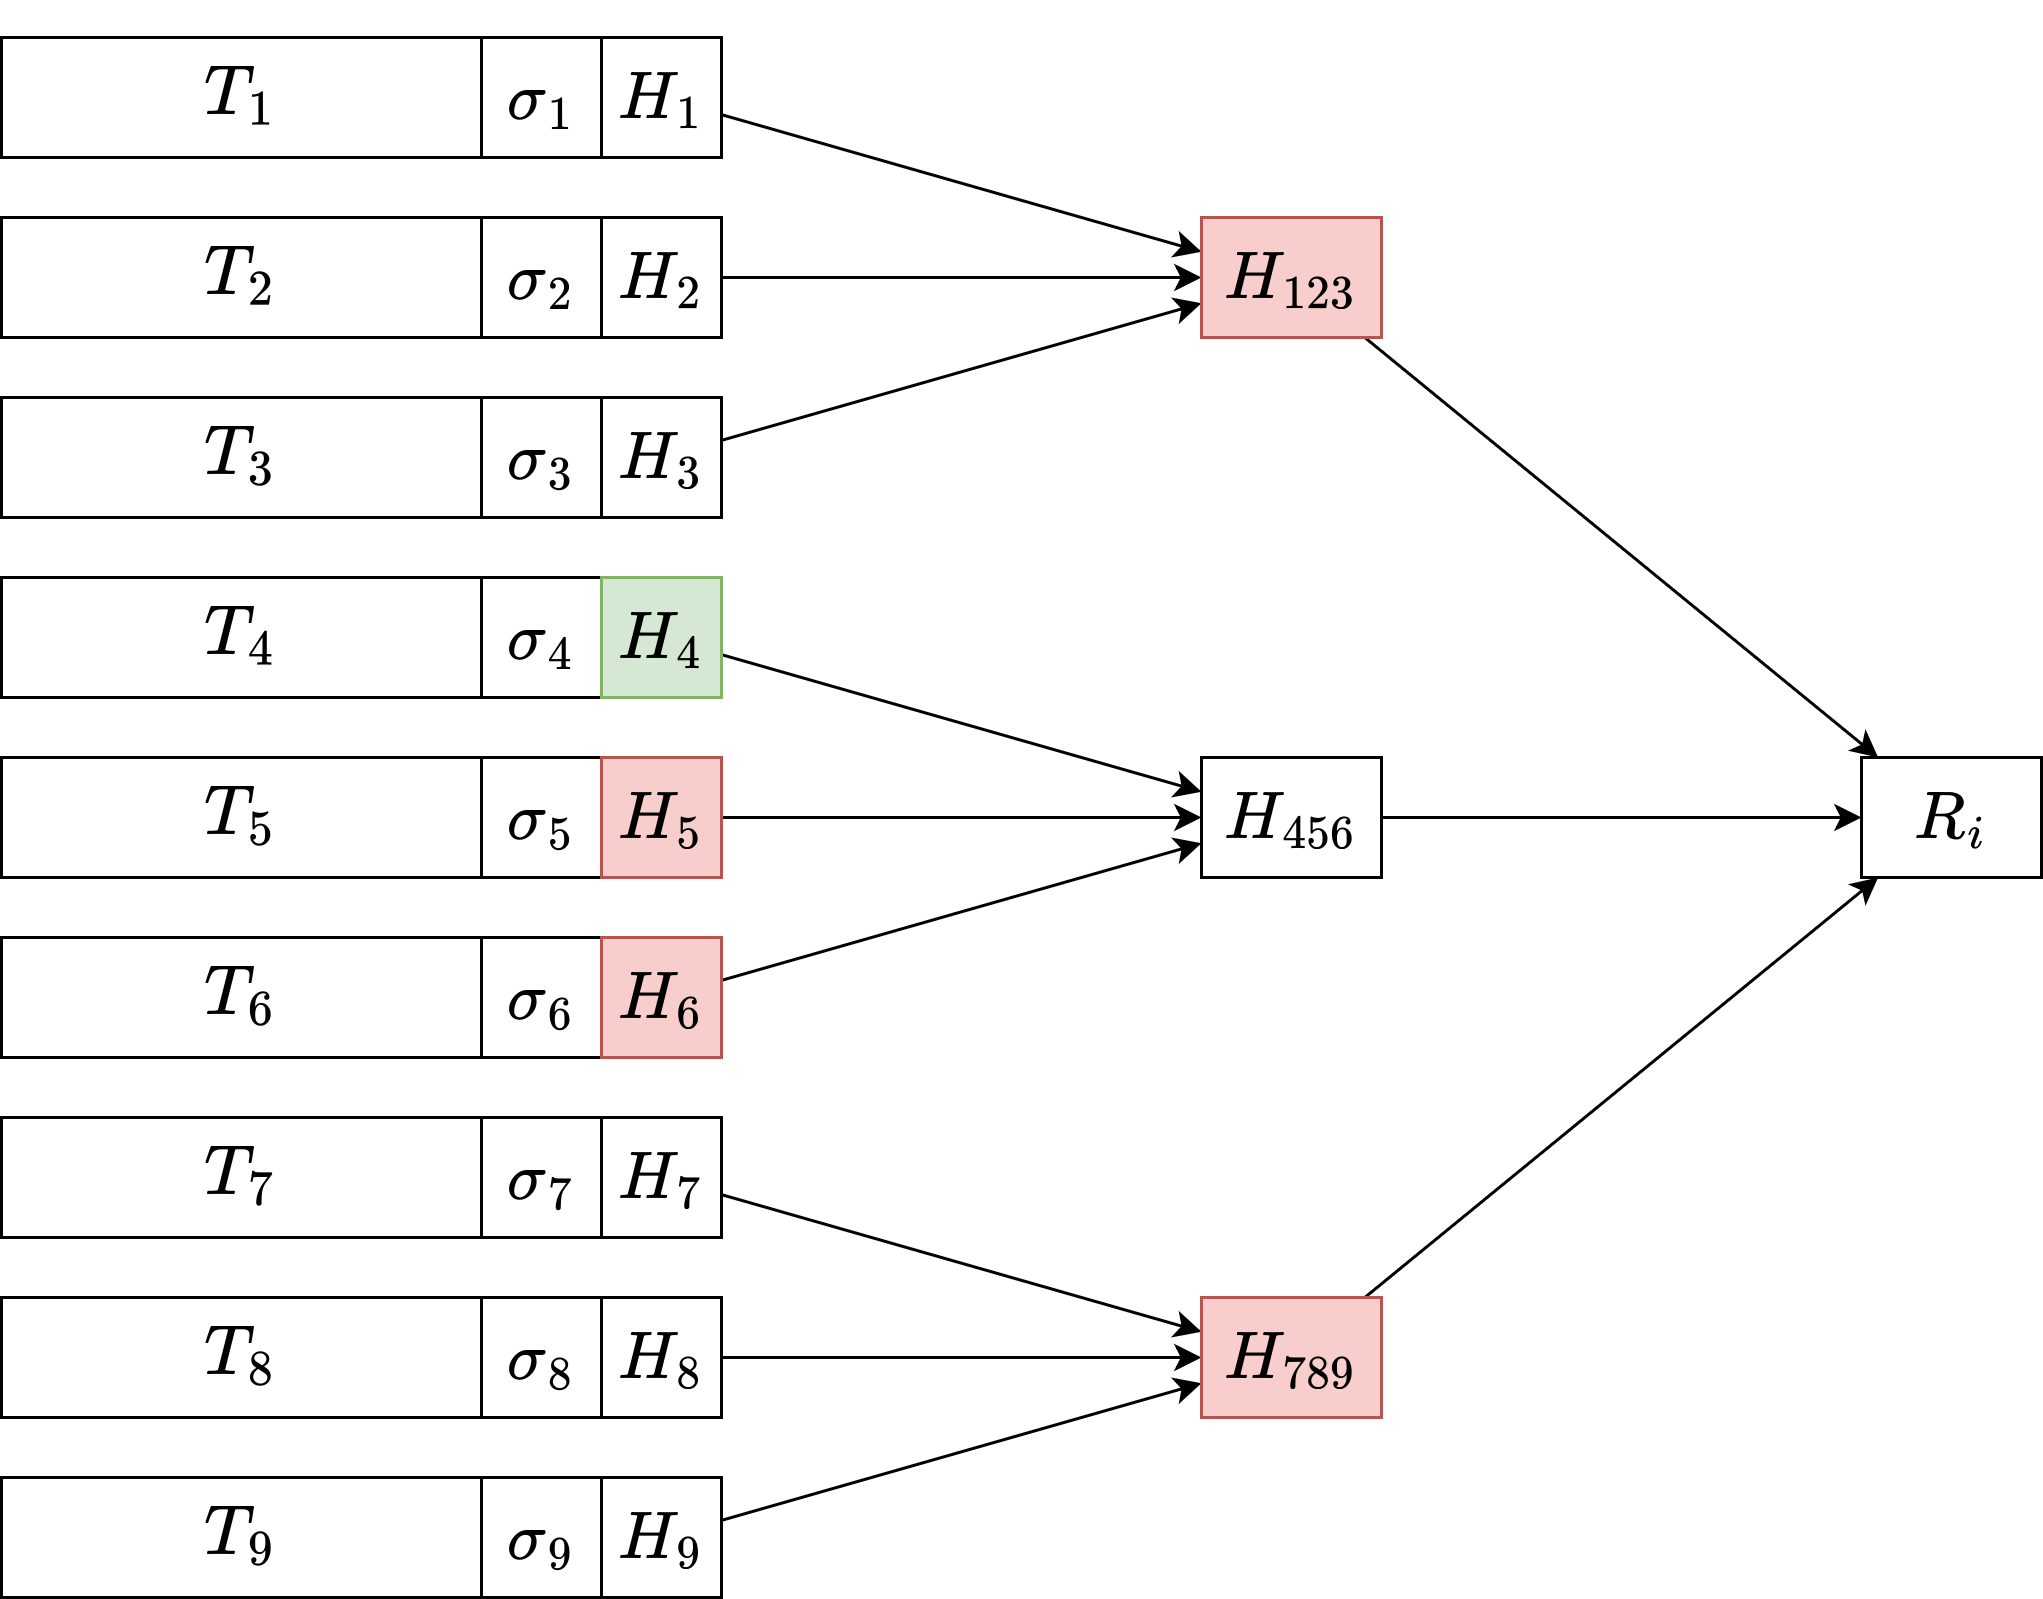
\includegraphics[width=\textwidth]{2.1.png}
            \caption{Схема вычисления хэша при помощи троичного дерева Меркла}
            \label{fig:2.1}
        \end{figure}
        
        Для того, чтобы доказать вхождение транзакции $T_4$ (хэш которой выделен зеленым на рисунке
        \ref{fig:2.1}) требуется предоставить Борису следующие значения: $H_5$, $H_6$ (соседние
        хэши) и $H_{123}$, $H_{789}$ (хэши соседних поддеревьев). Данные значения на рисунке
        \ref{fig:2.1} выделены красным.
        
        Борис вычисляет $\tilde{H}_{456}$ на основе известного $H_4$ и предоставленных $H_5$, $H_6$
        ($\tilde{H}_{456} = H(H_4 || H_5 || H_6)$), после чего на основе полученного значения и
        предоставленных $H_{123}$, $H_{789}$ рассчитывает $\tilde{S} = H(H_{123} || \tilde{H}_{456}
        || H_{789})$. Если $\tilde{S} = R_i$, то $T_4$ содержится в блоке (при условии, что все 
        предоставленные хэши верны, что было бы логично при доказательстве).
    \item Отметим, что путь от корня до проверяемой вершины содержит $\lceil \log_k n \rceil$
        элементов дерева. Для каждого элемента необходимо предоставить $k - 1$ хэш --- это
        хэши соседних поддеревьев (а для листового уровня --- соседние хэши-листы). Таким
        образом получается следующая формула для длины доказательства: 
        \begin{equation}
            (k - 1) \cdot \lceil \log_k n \rceil.
        \end{equation}
        
        \Answer{$(k - 1) \cdot \lceil \log_k n \rceil$}.
    \item Ясно, что для $x > 1$ выполнено: $\log_2 x < 2 \cdot \log_3 x$. Более наглядно это
        представлено на рисунке \ref{fig:2.3}:
        \begin{figure}[h!]
            \centering
            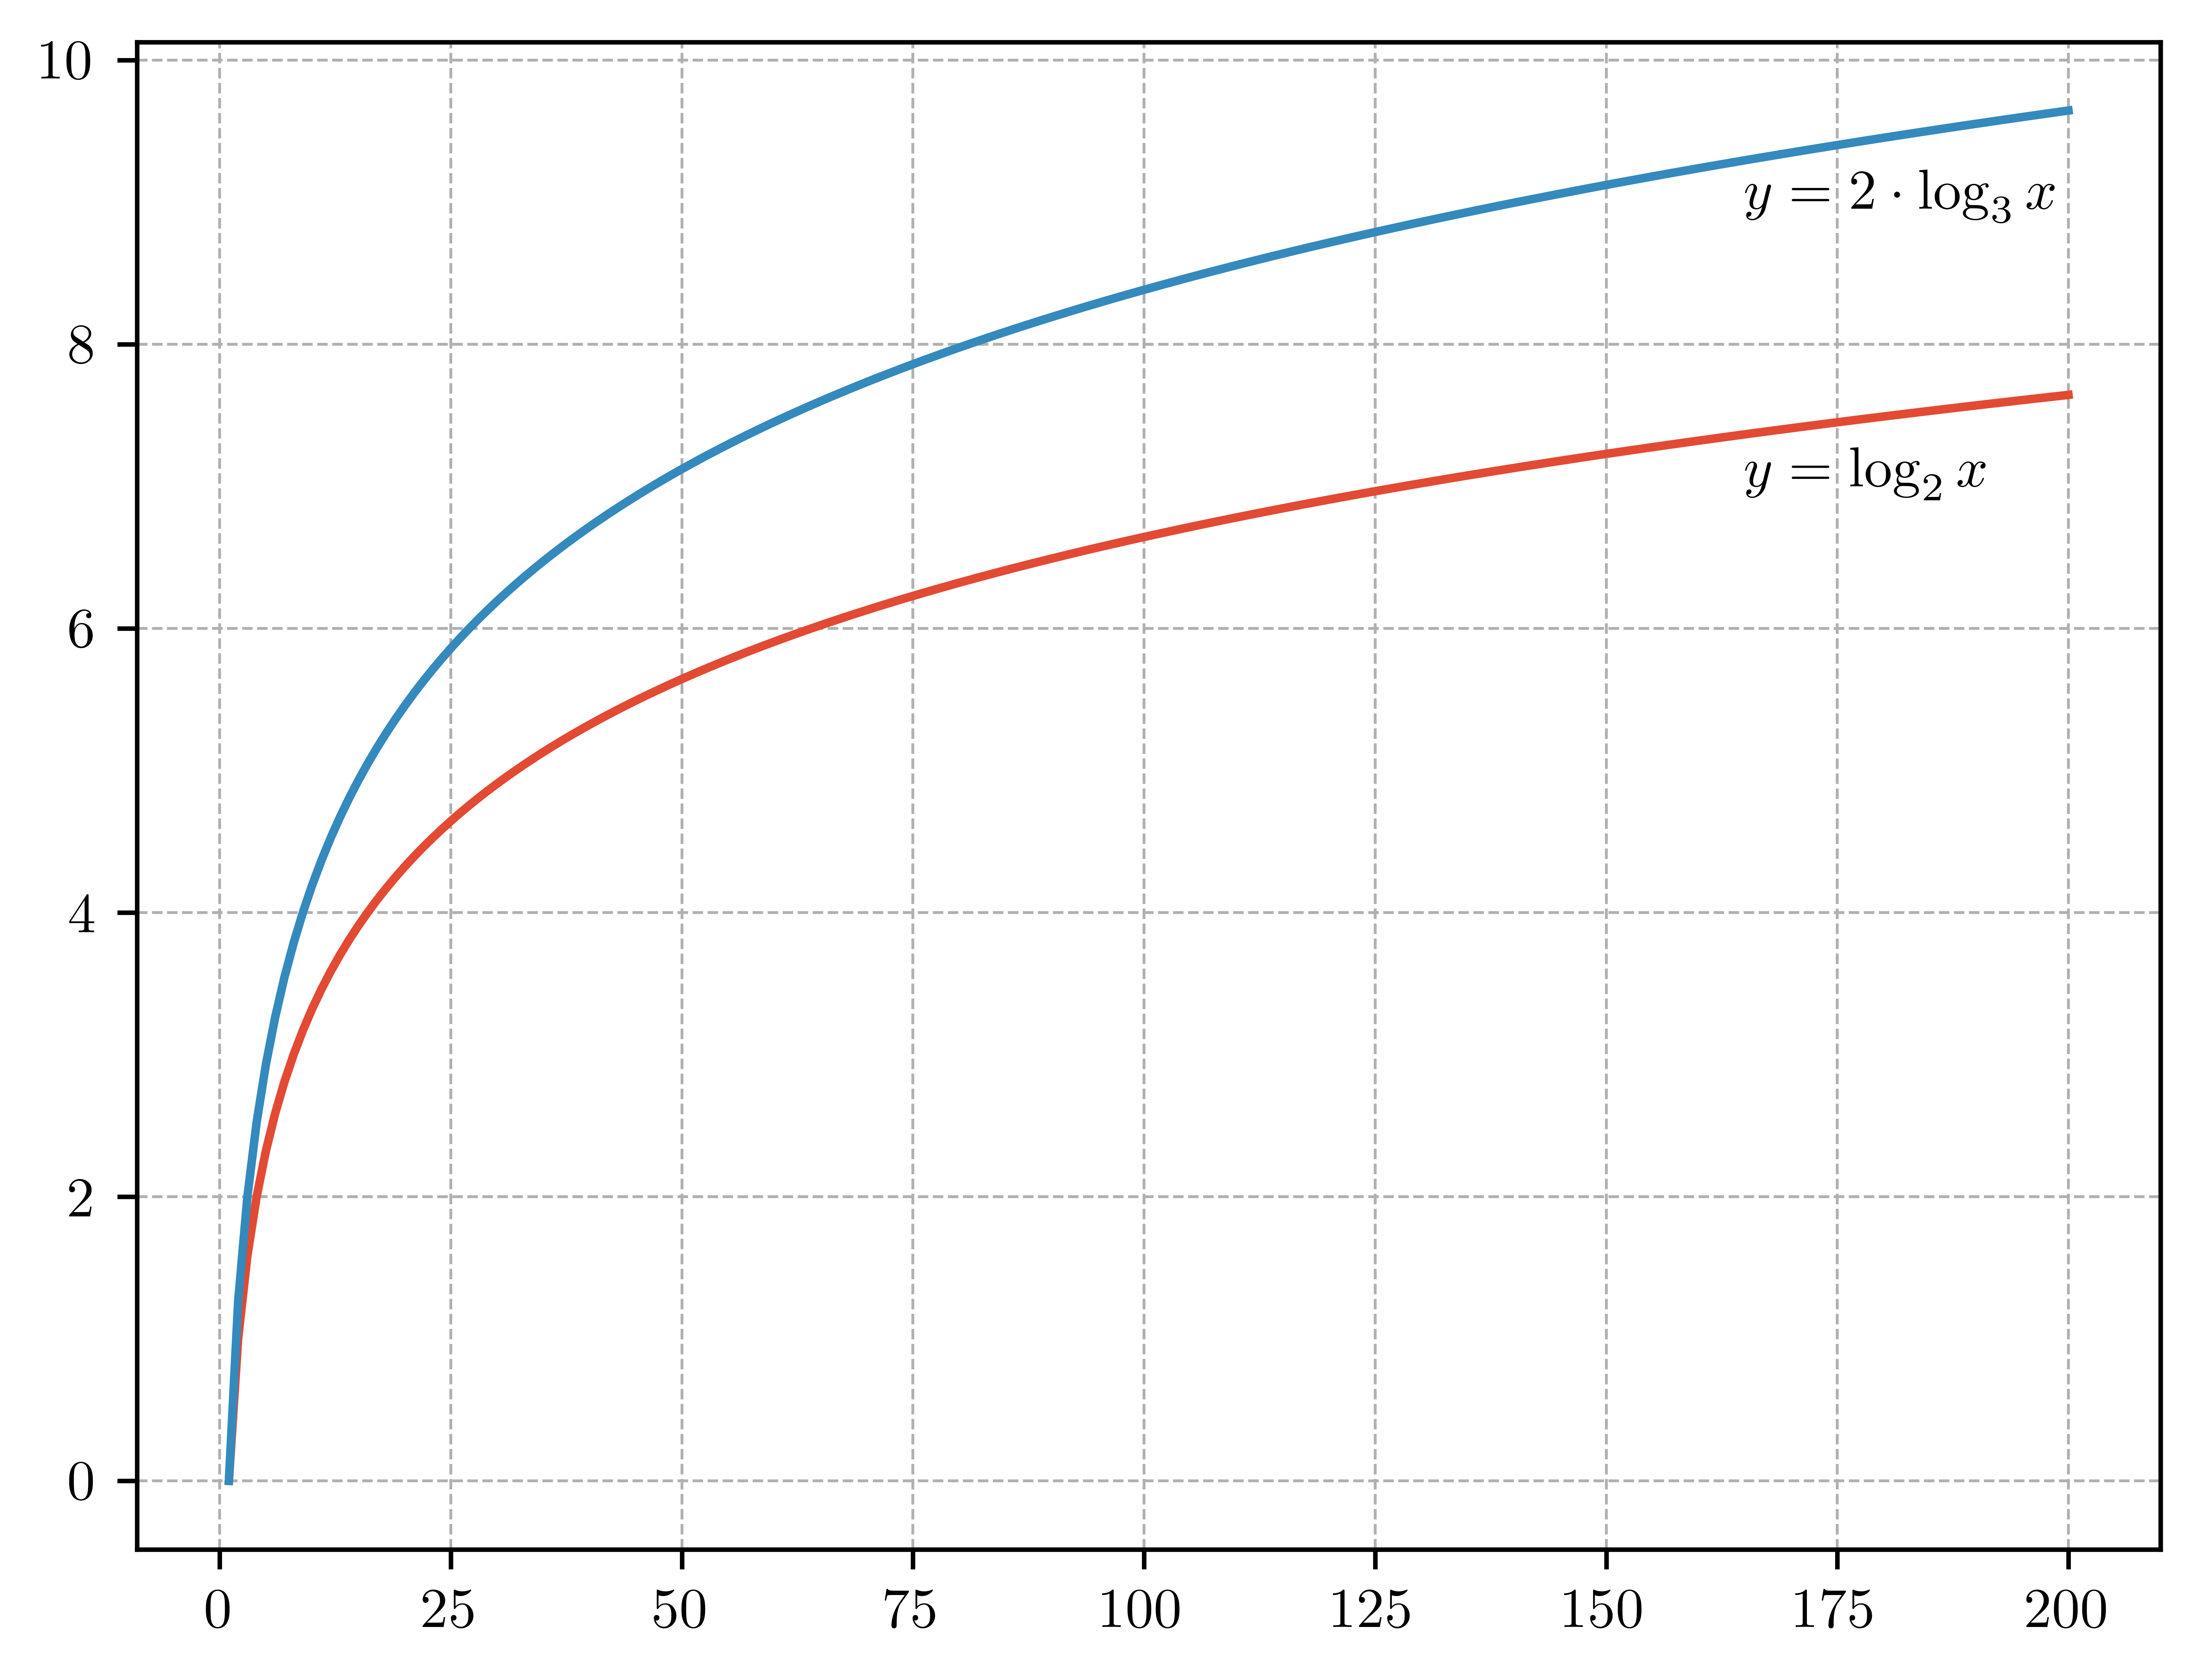
\includegraphics[width=0.7\textwidth]{2.3.png}
            \caption{графики двоичного (красная линия) и удвоенного троичного (синяя линия) 
                логарифмов в одинаковом масштабе}
            \label{fig:2.3}
        \end{figure}
        
        Из этого следует, что использование двоичного дерева Меркла эффективнее, чем троичного (и на 
        самом деле какого-бы то ни было еще), так как длина доказательства для него будет меньше.
        
        \Answer{двоичное дерево использовать оптимальнее, чем троичное}.
\end{enumerate}

\mysection{Задание 3}

\pagebreak
\mysection{Задание 4}

\pagebreak
\mysection{Задание 5}

\pagebreak
\mysection{Задание 6}

\pagebreak
\mysection{Задание 8}

\pagebreak
\mysection{Задание 9}

\end{document}
